\section{Shellcode}
\subsection{Definition}
Um das folgende Beispiel besser zu verstehen, sollte zunächst erklärt werden, was genau Shellcode ist und wofür er benutzt wird.
Shellcode ist definiert als eine Folge von Anweisungen, die über einen Exploit in einen Prozess injiziert und
dann durch diesen ausgeführt werden. Er wird verwendet, um die Funktionalität eines Prozesses zu verändern und
Befehle auf einem Zielsystem auszuführen. In der Computersicherheit bedeutet Shellcoding im ursprünglichen Sinne,
das Schreiben von Code, der bei der Ausführung eine Remote-Shell öffnet. Die Bedeutung von Shellcode hat sich jedoch weiterentwickelt und
beschreibt mittlerweile jeden Byte-Code, der in einen Exploit eingefügt wird, um eine gewünschte Aufgabe zu erfüllen.

Zwar ist es theoretisch möglich Shellcode in höheren Programmiersprachen zu schreiben, in der Praxis ist die effizienteste und
fast ausschließlich verwendete Sprache jedoch Assembly. Dies ermöglicht, so maschinennah wie möglich zu arbeiten,
um mehr Kontrolle über Abläufe zu haben und Speichergröße zu sparen. Der verfügbare Speicher für Shellcode ist meist limitiert.
Da Shellcode in Assembly geschrieben wird, ist es wichtig zu beachten, auf welcher Hardware und auf welchem Betriebssystem dieser laufen soll.
Es bestehen klare Unterschiede zwischen Linux- und Windows Shellcode: Unter Linux hat man überwiegend direkten Zugriff auf Interface und Kernel,
was unter Windows in der Regel nicht möglich ist. Im Folgenden wird ein Shellcode-Beispiel für 64Bit Unix Systeme betrachtet. \cite{tutorial1}

\subsection{Beispiel}
\begin{figure}[h]
    \centering
    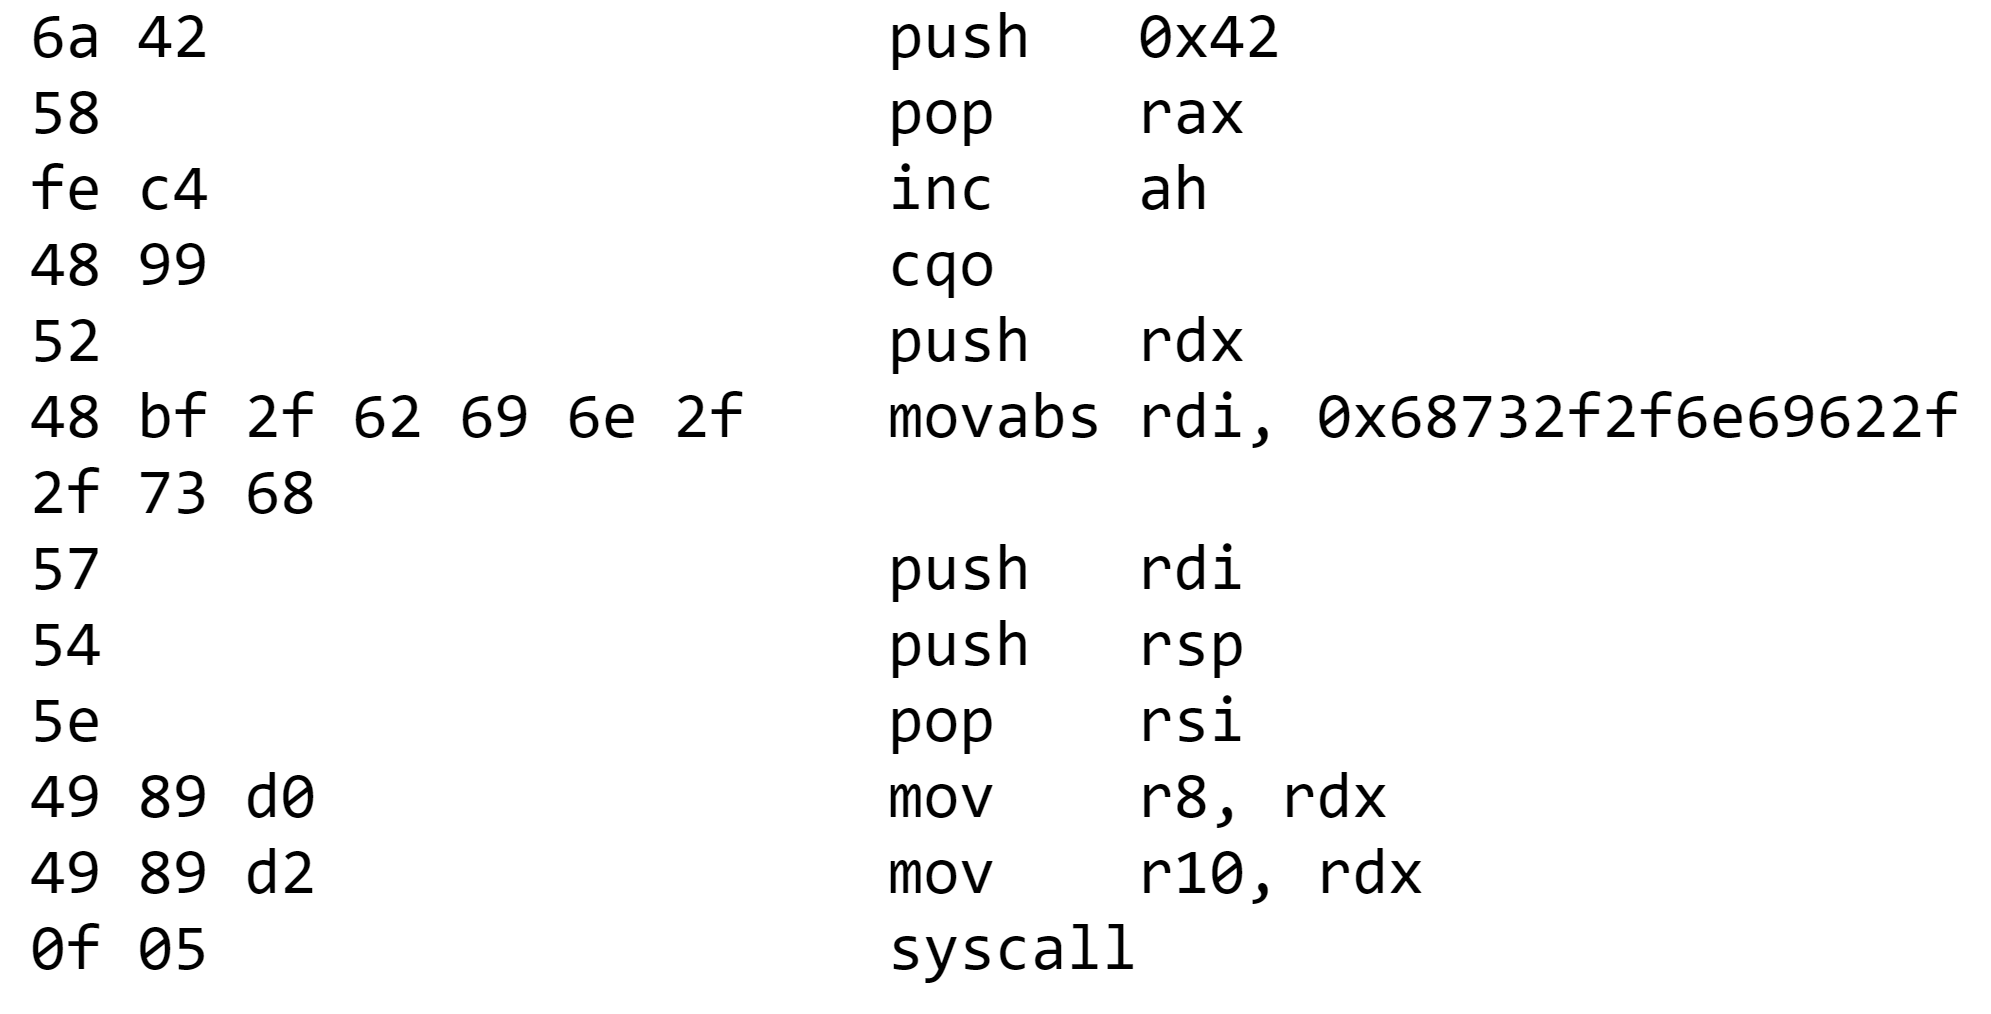
\includegraphics[width=0.9\textwidth,height=0.75\textheight,keepaspectratio]{images/shellstorm.png}
    \caption{Shellcode}
\end{figure}
\cite{shellstorm}

%TODO: Einfügen aus DC
%Struktur:
%Der syscall wird abgeschickt, vorher müssen einige Werte gesetzt werden um execveat aufzurufen



RAX -> system call number (322)
RDI -> first argument (path)
RSI -> second argument (pointer to path)
RDX -> third argument (0)
R10 -> fourth argument(0)
R8 -> fifth argument(0)
R9 -> sixth argument (not used) (Bearbeitet)


Bei dem folgenden Bild sieht man ein Beispiel zu einem Shellcode der dann wenn man
%!!!
vorhat ausgeführt werden kann um ein System zu manipulieren.Dieses ist aber einfach
gehalten um einen übersichtlicheren Blick zu bekommen. Daher sollte man hier von unten
beginnen. Der System Call wird aufgerufen und geht an die Adresse im Register RAX.
Dieser wurde mit der Hexadezimalzahl 0x42 belegt die auf den Stack gepusht
war und durch das pop da eingespeichert wurde, wichtig hierbei ist dass,
danach das Register ah was ein 8 Bit Teil vom 64 Bit Register RAX ist inkrementiert wird.
Mit anderen Worten wird der Wert 0x42 zum Wert 0x142 dieser ist in
Dezimalzahlen 322.Also geht der  System Call an die Nummer 322.
Der nächste Schritt des Aufrufs ist es ans Register RDI zu gehen was das first
argument enthält und den path darstellt. Im Code sehen wir das durch den
Befehl movabs der String ("/bin//sh") als Hexadezimalzahl ins Register
verschoben wird und danach durch den push Befehl auf dem Stack ist.
Der dritte Schritt ist dass, der Aufruf sich das second argument anguckt
was den Weg zum path hat und im Register RSI enthalten ist. Das besondere
Register RSP oder auch stack pointer zeigt auf den Pfad der letzten Adresse
in dem falle den von RDI und dieser Pfad wird in RSI gespeichert, daher die
Befehle push RSP und pop RSI. Der Rest vom Code ist in diesem falle nicht so
wichtig aber durch den Befehl cqo(convert word to Quadword) am Anfang wird das
Register RDX auf null gesetzt und diesen Wert übernehmen dann auch die zwischen
Register R8 und R10 durch den mov Befehl. Einen wirklichen nutzen hat dieser
kleine 29 Byte große
Shellcode nicht, aber er zeigt hervorragend wie man die Register mit dem der
Kernel durch den System Call arbeitet man manipulieren kann.
